\section{16-bit addition using direct addressing mode}
\subsection{Aim}
To add two 16-bit numbers using direct addressing mode

\subsection{Code}
\begin{lstlisting}
DATA SEGMENT
    sum DW ?
ENDS DATA

CODE SEGMENT
ASSUME DS:DATA, CS:CODE
START:
    MOV AX, DATA
    MOV DS, AX
    MOV [1000H], 100
    MOV [1002H], 200
    MOV AX, [1000H]
    MOV BX, [1002H]
    ADD AX, BX
    MOV [sum], AX
    MOV AH, 04CH
    INT 21H
CODE ENDS
END START
\end{lstlisting}

\subsection{Output}
\begin{center}
	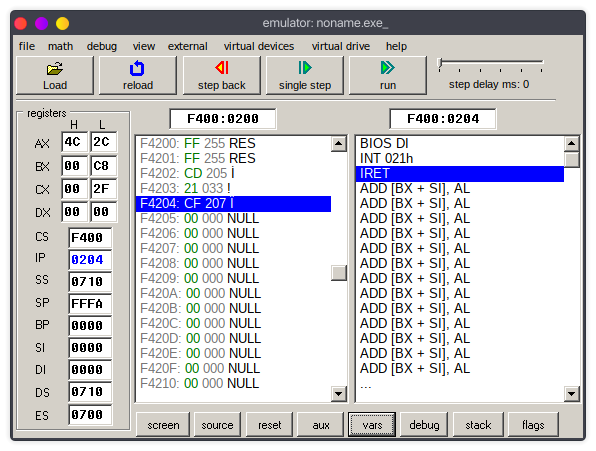
\includegraphics[width=0.90\textwidth]{img/p1/ss1.png}
	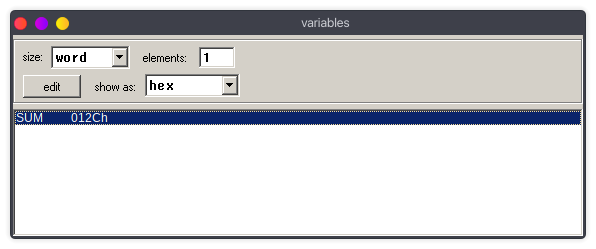
\includegraphics[width=0.90\textwidth]{img/p1/ss2.png}
\end{center}

\subsection{Result}
Two 16 bit numbers were added using direct addressing mode in emu8086 and output was verified